\documentclass{article}

%%%%%%%%%%%%%%%%%%%%%%%%%
% Packages & Macros
%%%%%%%%%%%%%%%%%%%%%%%%%

% For including graphics
\usepackage{graphicx}

% For title page
\usepackage{datetime}
\newdateformat{monthyeardate}{\monthname[\THEMONTH] \THEYEAR}

% For supporting linking
\usepackage{hyperref}
\hypersetup{colorlinks,urlcolor=blue,linkcolor=blue}

% For table colouring (in command line tables)
\usepackage{colortbl}

%%%%%%%%%%%%%%%%%%%%%%%%%
% Tool-Specific Macros
%%%%%%%%%%%%%%%%%%%%%%%%%
\usepackage{xspace}

\newcommand{\args}[1] {\textit{#1}}
\newcommand{\cmd}[1] {\texttt{#1}}     % Use for command window commands, e.g., \cmd{svn up}
\newcommand{\block}[1] {\textsf{#1}}   % Use for Simulink block names, e.g., \cmd{Subsystem1}
\newcommand{\signal}[1] {\textsf{#1}}   % Use for Simulink block names, e.g., \cmd{Subsystem1}
\newcommand{\ring}[1] {\textsf{#1}} 	 % Use for files names and paths
\newcommand{\keyword}[1] {\texttt{#1}} % Use for keywords of programming languages, e.g., \keyword{while}
\newcommand{\file}[1] {\texttt{#1}} 	 % Use for files names and paths
\newcommand{\param}[1] {\textsf{#1}}   % Use for block parameter names, e.g., \param{BlockType}

% Matlab Products
\newcommand{\matlab}{\textsc{Matlab}\@\xspace}
\newcommand{\Matlab}{\textsc{Matlab}\@\xspace}
\newcommand{\Simulink}{Simulink\@\xspace}
\newcommand{\simulink}{Simulink\@\xspace}
\newcommand{\SDV}{Simulink Design Verifier\@\xspace}
\newcommand{\mpath}{\Matlab search path\@\xspace}

% Block Names (not BlockType)
\newcommand{\ds}{\block{Data Store}\@\xspace}
\newcommand{\DSM}{\block{Data Store Memory}\@\xspace}
\newcommand{\DSR}{\block{Data Store Read}\@\xspace}
\newcommand{\DSW}{\block{Data Store Write}\@\xspace}
\newcommand{\DSRW}{\block{Data Store Read/Write}\@\xspace}
\newcommand{\DSMRW}{\block{Data Store Memory/Read/Write}\@\xspace}

\newcommand{\goto}{\block{Goto}\@\xspace}
\newcommand{\from}{\block{From}\@\xspace}

\newcommand{\inport}{\block{Inport}\@\xspace}
\newcommand{\outport}{\block{Outport}\@\xspace}
\newcommand{\constant}{\block{Constant}\@\xspace}
\newcommand{\ground}{\block{Ground}\@\xspace}
\newcommand{\subsystem}{\block{Subsystem}\@\xspace}

\newcommand{\logic}{\block{Logical Operator}\@\xspace}
\newcommand{\relational}{\block{Relational Operator}\@\xspace}
\newcommand{\ifblk}{\block{If}\@\xspace}
\newcommand{\switch}{\block{Switch}\@\xspace}
\newcommand{\merge}{\block{Merge}\@\xspace}

\newcommand{\docblock}{\block{DocBlock}\@\xspace}

\newcommand{\simfunc}{\block{Simulink Function}\@\xspace}
\newcommand{\simfunccaller}{\block{Function Caller}\@\xspace}

\newcommand{\toworkspace}{\block{To Workspace}\@\xspace}
\newcommand{\fromworkspace}{\block{From Workspace}\@\xspace}

\newcommand{\tofile}{\block{To File}\@\xspace}
\newcommand{\fromfile}{\block{From File}\@\xspace}

\newcommand{\fromspreadsheet}{\block{From Spreadsheet}\@\xspace}

\newcommand{\modelref}{\block{Model Reference}\@\xspace}
\newcommand{\library}{\block{Library}\@\xspace}
\newcommand{\librarylink}{\block{Library Link}\@\xspace}

% Commonly used parameters
\newcommand{\AND}{\param{AND}\@\xspace}
\newcommand{\OR}{\param{OR}\@\xspace}
\newcommand{\NOT}{\param{NOT}\@\xspace}
\newcommand{\NOR}{\param{NOR}\@\xspace}
\newcommand{\NAND}{\param{NAND}\@\xspace}
\newcommand{\XOR}{\param{XOR}\@\xspace}
\newcommand{\NXOR}{\param{NXOR}\@\xspace}

% Common Abbreviations
% Example
\newcommand{\eg}{\textrm{e.g.,}\@\xspace}

% That Is To Say
\newcommand{\ie}{\textrm{i.e.,}\@\xspace}

% And So On
\newcommand{\etc}{\textrm{etc.}\@\xspace}

% And Others
\newcommand{\etal}{\textrm{et al.}\@\xspace}

% With Respect To
\newcommand{\wrt}{\textrm{w.r.t.}\@\xspace}

% Vice Versa
\newcommand{\vrsa}{\textrm{vice versa}\@\xspace}

% Symbols

\usepackage{amssymb}
\newcommand{\checkbox}{\makebox[0pt][l]{$\square$}\raisebox{.15ex}{\hspace{0.1em}$\checkmark$}}%
\newcommand{\uncheckbox}{$\square$~}%


\newcommand{\ToolName}{Data Store Rescope Tool\@\xspace}

\newcommand{\menu}[2]{%
	\ifthenelse{\equal{#1}{1}}{Rescope All}{}%
  	\ifthenelse{\equal{#1}{2}}{Rescope Selected}{}%
  	\ifthenelse{\equal{#1}{3}}{Rescope Non-Selected}{}%
}

\newcommand{\func}[2]{%
	\ifthenelse{\equal{#1}{1}}{dataStoreRescope}{}%
  	\ifthenelse{\equal{#1}{2}}{rescopeSelected}{}%
}

\newcommand{\toolFolder}{\cmd{DataStoreRescope}}
\newcommand{\demoName}{\cmd{DataStoreRescopeDemo}\@\xspace}

\newcommand{\FCA}{0} 	% Enable/disabled FCA-specific content	
%\newcommand{\HowSetPath}{\ifthenelse{\equal{\FCA}{1}}{If it is not, go to \cmd{File~>~Set~Path...}, press \cmd{Add with Subfolders}, and select the \cmd{McMaster\_Tools} folder. Restart \matlab after doing so.}{}}

%%%%%%%%%%%%%%%%%%%%%%%%%
% Document
%%%%%%%%%%%%%%%%%%%%%%%%%

\begin{document}

%%%%%%%%%%%%%%%%%%%%%%%%%%%%%%%%%%%%%%%%%%%%%%%%%%%%%%%%%%%%%%%%%%%
% Title Page
%%%%%%%%%%%%%%%%%%%%%%%%%%%%%%%%%%%%%%%%%%%%%%%%%%%%%%%%%%%%%%%%%%%
\title{\ToolName}
\date{\monthyeardate\today}
\maketitle
\vfill

\begin{figure}
	\centering
	
\includegraphics[]{../../common/McSCert_Logo.pdf} \\
	McMaster Centre for Software Certification (McSCert)
\end{figure}

\newpage

%%%%%%%%%%%%%%%%%%%%%%%%%%%%%%%%%%%%%%%%%%%%%%%%%%%%%%%%%%%%%%%%%%%
% Introduction
%%%%%%%%%%%%%%%%%%%%%%%%%%%%%%%%%%%%%%%%%%%%%%%%%%%%%%%%%%%%%%%%%%%
\section{Introduction}

% Briefly, what is the tool?
% Provide any background or references.
The \ToolName is used to properly scope \DSM blocks in \Simulink models. The tool aims to assist software development actives, as well as software refactoring and maintenance.

Using \DSM blocks higher in the model hierarchy than needed is bad software engineering practice, and is similar to using global variables in programming. This can result in inadvertent/unwanted access to the memory, and also clutters the interface of subsystems by showing low-level details. The \ToolName is used on \DSM blocks in order to push them down to the lowest layer possible, while still in scope of their corresponding \DSR and \DSW blocks in the model.

This tool can also repair the scope of a \DSM block when it is positioned too low in the hierarchy, such that its \DSR or \DSW blocks are out of its scope. In this case, the \DSM block is repositioned higher in the hierarchy.

% Is there more information?
\subsection*{More Information}
For more information on the tool and how it can be used in a model-based development with \Simulink, please refer to the following papers:

\vspace{1em}
Vera Pantelic, Steven Postma, Mark Lawford, Monika Jaskolka, Bennett Mackenzie, Alexandre Korobkine, Marc Bender, Jeff Ong, Gordon Marks, Alan Wassyng, \href{https://link.springer.com/article/10.1007/s10009-017-0450-9}{``Software engineering practices and Simulink: bridging the gap,"} \textit{International Journal on Software Tools for Technology Transfer (STTT)}, 2017, 1-23.

\vspace{1em}
Vera Pantelic, Steven Postma, Mark Lawford, Alexandre Korobkine, Bennett Mackenzie, Jeff Ong, and Marc Bender, \href{http://www.cas.mcmaster.ca/~lawford/papers/MODELSWARD2015.pdf}{``A Toolset for Simulink: Improving Software Engineering Practices in Development with Simulink,"}\textit{Proceedings of 3rd International Conference on Model-Driven Engineering and Software Development (MODELSWARD 2015)}, SCITEPRESS, 2015, 50--61.

\newpage
%%%%%%%%%%%%%%%%%%%%%%%%%%%%%%%%%%%%%%%%%%%%%%%%%%%%%%%%%%%%%%%%%%%
% How to Use the Tool
%%%%%%%%%%%%%%%%%%%%%%%%%%%%%%%%%%%%%%%%%%%%%%%%%%%%%%%%%%%%%%%%%%%
\section{How to Use the Tool}
This section describes what must be done to setup the \ToolName, as well as how to use the tool.

%---------------------------------------
% What needs to be done before the tool can be used? 
% What needs to be done to a model in order for it to work on said model?
%---------------------------------------
\subsection{Prerequisites and Installation}

\begin{enumerate}
  \item Use \Matlab/\Simulink 2011b or newer.
	\item To install the tool,
	\begin{enumerate}
		\item from a \file{.zip} file --- unzip the contents into your desired location. Ensure the unzipped folder and subfolders are present in your \mpath, or add them if they are not present. Run \href{https://www.mathworks.com/help/simulink/ug/registering-customizations.html}{sl\_refresh\_customizations} to refresh the Context Menu. 
		\item from a \file{.mltbx} file --- simply open \Matlab and double-click on the file. Your \mpath should be automatically configured.
		\item from the files only --- add the folders and subfolders to your \mpath. Run \href{https://www.mathworks.com/help/simulink/ug/registering-customizations.html}{sl\_refresh\_customizations} to refresh the Context Menu.
	\end{enumerate}
	\begin{itemize}
		\item \textit{Note:} If running the command ``\cmd{which dataStoreRescope}'' indicates that the script is not found, then the tool needs to be added to the \mpath.
		For information on adding files to the \mpath, please see the \href{https://www.mathworks.com/help/matlab/matlab_env/add-remove-or-reorder-folders-on-the-search-path.html}{MathWorks documentation}.
	\end{itemize}
	\item Ensure your model is open and unlocked.
\end{enumerate}

%---------------------------------------
% How/when do you access the tool?
%---------------------------------------
\subsection{Getting Started}
The \ToolName can be used via the \Simulink Context Menu, which can be viewed by right-clicking in a model. The following options can be available in the \ToolName menu, depending on what is selected in the model. These options are shown in Figure~\ref{FIG:contextMenu}.
\begin{itemize}
	\item \emph{\menu{1}} --- Available at all times.
	\item \emph{\menu{2}} --- Available when one or more \DSM, \DSR, or \DSW blocks are selected.
	\item \emph{\menu{3}} --- Available when one or more \DSM, \DSR, or \DSW blocks are selected.
\end{itemize}

\begin{figure}[htb]
	\centering
	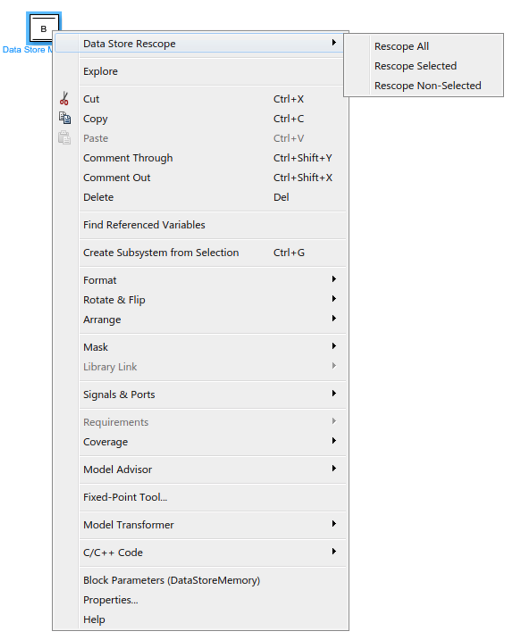
\includegraphics[width=0.7\textwidth]{../figs/ContextMenu}
	\caption{\Simulink Context Menu with tool options visible.}
	\label{FIG:contextMenu}
\end{figure}

%---------------------------------------
% What are the main uses of the tool?
%---------------------------------------
\newpage
\subsection{Functionality}
This section describes the tool functionality when being used from the \Simulink Context Menu (Figure~\ref{FIG:contextMenu}).

\subsubsection*{\menu{1}}
Right-clicking anywhere in the model and selecting \cmd{\menu{1}} will move up/down all \DSM blocks starting from the root level of the model. They are each moved to their lowest level of the hierarchy such that all references to them via \DSRW blocks are still within scope. 

\subsubsection*{\menu{2}}
Selecting one or more \DSM blocks, and then selecting \cmd{\menu{2}} will move up/down the selected \DSM blocks only. They are each moved to their lowest level of the hierarchy such that all references to them via \DSRW blocks are still within scope. All other non-selected \DSM blocks remain in their original location.

\subsubsection*{\menu{3}}
Selecting one or more \DSM blocks, and then selecting \cmd{\menu{3}} will move up/down all \DSM blocks, except those which are selected. Those not selected are moved to their lowest level of the hierarchy such that all references to them via \DSRW blocks are within scope.

%---------------------------------------
% What are the configuration options for the tool?
%---------------------------------------
\subsection{Configuration Parameters}
The configuration file \cmd{config.txt} is included in \cmd{\toolFolder\textbackslash src}. The following configuration parameters are utilized by the tool, and can be modified by the user in order to tailor tool functionality:

\begin{itemize}
	\item \cmd{linkedBlocksEnabled} --- Enables or disables the ability to rescope \DSM blocks inside linked subsystems.
\end{itemize}

Please see the configuration file for more details regarding parameter usage and accepted values. These parameters can be modified with \matlab open, and do not require that \matlab be restarted for the changes to take effect.

%---------------------------------------
% What else does the tool do?
%---------------------------------------
\subsection{Logs}
When invoking any of the tool options, a log text file is created to summarize the changes in the model. This text file will be created in the same directory as the model on which the operation was performed, and will be named \texttt{modelName\_RescopeLog.txt}. If a previous log file already exists in this location, subsequent log content will be appended to the file. The log file includes the following information:

\begin{itemize}
	\item Data and time the rescope operation was performed
	\item Total number of \DSM blocks in the model
	\item Total number of \DSM blocks rescoped
	\item Percentage of \DSM blocks rescoped
	\item A list of all \DSM blocks rescoped, including:
	\begin{itemize}
		\item Block name
		\item Initial location in the model
		\item New location in the model
	\end{itemize}
\end{itemize}

\subsection{Errors and Warnings}
Any errors or warnings during tool use will be visible in the \matlab Command Window. Errors will be shown when the model is locked or function parameters are incorrect.  

Warnings will be given if the operation has completed successfully, however the user should be made aware of a situation which may or may not need further attention. For example, at different levels of the hierarchy, \DSM blocks can have the same name. Given that the default names  are ``\block{Data Store Memory}", ``\block{Data Store Memory1}", ``\block{Data Store Memory2}", etc., and if the user does not change them, it may be the case that multiple \DSM blocks, located in different subsystems, have the same name. As a result, when rescoping is performed, two or more \DSM blocks of the same name may be placed in the same subsystem, resulting in an error. Therefore, the conflicting blocks will be renamed, following the usual \Simulink convention described earlier. The user will be notified of this via a warning.

%%%%%%%%%%%%%%%%%%%%%%%%%%%%%%%%%%%%%%%%%%%%%%%%%%%%%%%%%%%%%%%%%%%
% Example
%%%%%%%%%%%%%%%%%%%%%%%%%%%%%%%%%%%%%%%%%%%%%%%%%%%%%%%%%%%%%%%%%%%
\clearpage
\section{Example}

Use the command \demoName in the \Simulink Command Window to open the example model, shown\footnote{As there are 5 hierarchical levels, we do not show them all here.} in Figure~\ref{FIG:demo1}. There are three \DSM blocks in this example: \block{B} and \block{C} at the root level, and \block{A} at the second level of the hierarchy. These three \DSM blocks are used throughout the models in various locations:

\begin{itemize}
	\item Although they are in the root level, \block{B} and \block{C} are used lower in the hierarchy at levels 3 and 4, respectively. Therefore, \DSM \block{B} and \block{C} are located higher than they need to be in the model, and can be moved downwards.
	\item \DSW \block{A} is at the root level, however, \DSM \block{A} is located below it in the hierarchy, at level 2. This will result in an error upon simulation. To repair this, \DSM \block{A} should be placed at the root level, so that it is within the scope of \DSW \block{A}.
\end{itemize}

To to rescope all possible \DSM blocks correctly, right-click anywhere in the model and select the \cmd{\menu{1}} option. The resulting model is shown$^1$ in Figure~\ref{FIG:demo2}. \DSM blocks \block{B} and \block{C} were moved down in the hierarchy, while \block{A} was moved up to the root.

It is also possible to right-click on each of the \DSM blocks (or their associated \DSRW blocks) individually, and select the \cmd{\menu{2}} option to achieve the same result.

\begin{figure}
	\centering
	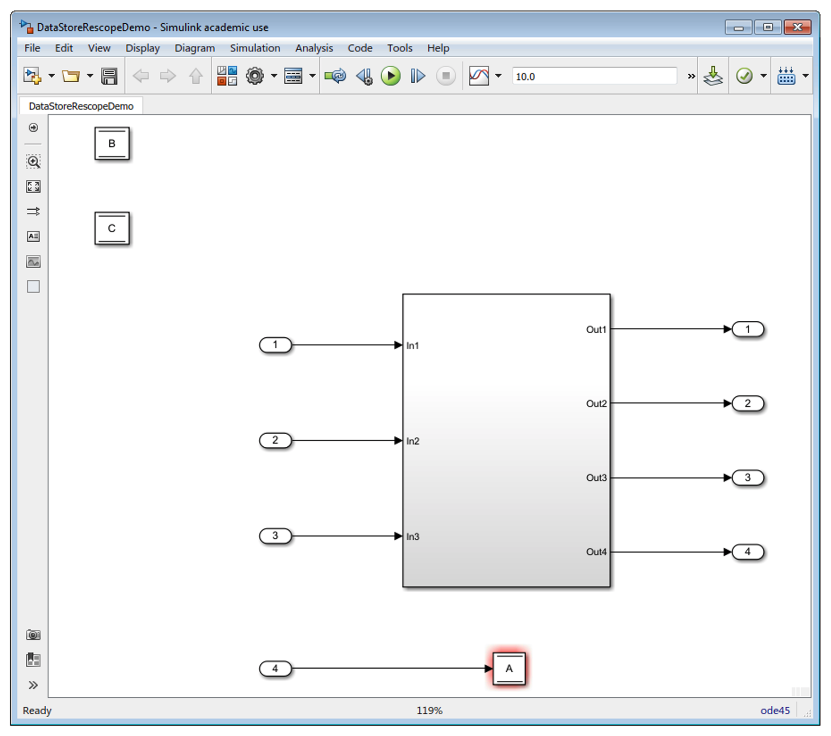
\includegraphics[width=0.8\textwidth]{../figs/Demo1}
	\caption{\ToolName demo model.}
	\label{FIG:demo1}
\end{figure}

\begin{figure}
	\centering
	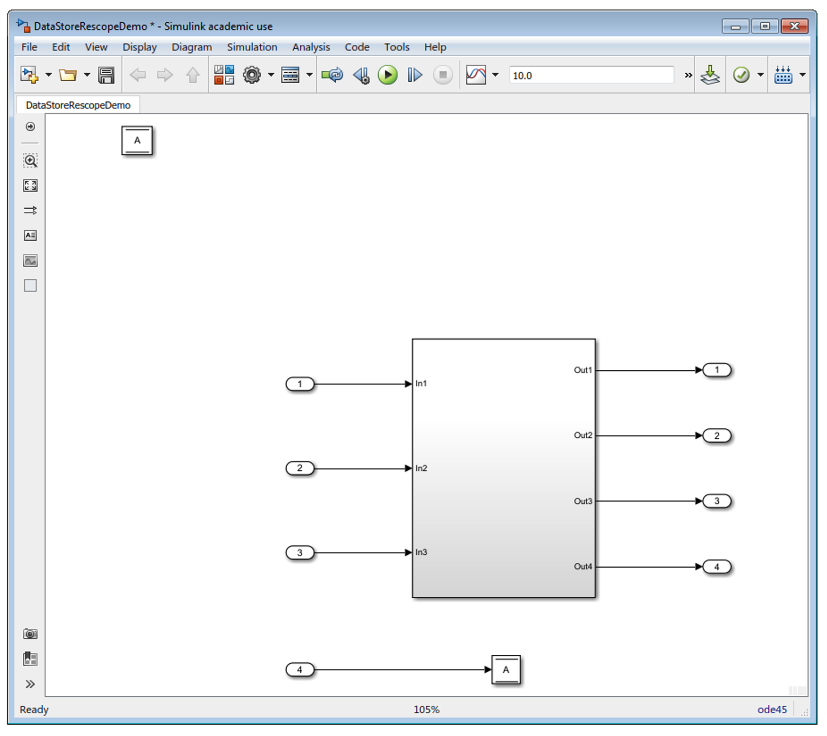
\includegraphics[width=0.8\textwidth]{../figs/Demo2}
	\caption{Resulting model after \cmd{Rescope All} operation.}
	\label{FIG:demo2}
\end{figure}

%%%%%%%%%%%%%%%%%%%%%%%%%%%%%%%%%%%%%%%%%%%%%%%%%%%%%%%%%%%%%%%%%%%
% Matlab Commands
%%%%%%%%%%%%%%%%%%%%%%%%%%%%%%%%%%%%%%%%%%%%%%%%%%%%%%%%%%%%%%%%%%%
\clearpage
\section{Matlab Commands}

The tool can also be used via the \matlab command line, with the following functions.

%---------------------------------------
% Command 1
%---------------------------------------
\begin{center}
	\begin{tabular}{| >{\columncolor[gray]{0.9}}l | p{8.5cm} |} \hline
		Function 		& \cmd{\func{1}} \\ \hline
		Syntax			& \cmd{\func{1}}(\args{model, dontMove}) \\ \hline
		Description		& Rescopes all \DSM blocks except for those listed in \args{dontMove}. \\ \hline
		Inputs	& \args{model}: The \Simulink model name (or top-level system name) of the model on which to perform the rescoping operation. \newline
						  \args{dontMove}: A cell array of \DSM pathnames which are not to be moved. \\ \hline
		Outputs			& N/A \\ \hline
	\end{tabular}
\end{center}

\paragraph{Example:} The following command moves all \DSM blocks in the open/loaded model \demoName to their proper level in the hierarchy such that \DSRW references remain within scope. The resulting model is shown as Figure~\ref{FIG:demo2}.

\begin{center}
	\cmd{\func{1}~(`\demoName', \{\})}
\end{center}

%---------------------------------------
% Command 2
%---------------------------------------
\begin{center}
	\begin{tabular}{| >{\columncolor[gray]{0.9}}l | p{8.5cm} |} \hline
		Function 		& \cmd{\func{2}} \\ \hline
		Syntax			& \cmd{\func{2}}(\args{model, dataStores}) \\ \hline
		Description	& Rescopes only specified \DSM blocks. \\ \hline
		Inputs				& \args{model}: The \Simulink model name (or top-level system name) of the model on which to perform the rescoping operation. \newline
						  	\args{dataStores}: A cell array of \DSM pathnames which are to be moved. \\ \hline
		Outputs			& N/A \\ \hline
	\end{tabular}
\end{center}

\paragraph{Example:} The following command moves \DSM blocks \block{A}, \block{B}, and \block{C} in the open/loaded model \demoName to their proper level in the hierarchy such that \DSRW references remain within scope. The resulting model is shown as Figure~\ref{FIG:demo2}.

\vspace{1em}
%\begin{center}
	\cmd{\func{2}~(`\demoName', \{`\demoName/Data Store Memory1', `\demoName/Data Store Memory2', \newline `\demoName/Subsystem/Data Store Memory'\})}
%\end{center}

\vspace{2em}
\textit{\textbf{Note:} \Simulink block names, such as for \block{Subsystem}s and \DSMRW, can contain newline characters. When using the command line functions, please ensure you include them in the pathnames of the \args{dontMove} and \args{dataStores} arguments.}


\end{document}